\documentclass[border=4pt]{standalone}
\usepackage{amsmath,amssymb,amsfonts}
\usepackage{xcolor,colortbl,array,booktabs,multirow}
\usepackage{tikz}
\usetikzlibrary{arrows, automata, backgrounds, calendar, chains, decorations,
    matrix, mindmap, patterns, petri, positioning, shadows, shapes.geometric,
    trees, shapes, decorations.pathreplacing, calc, tikzmark, arrows.meta}
\newcommand{\st}{\text{ s.t. }}
\newcommand{\x}{\mathbf{x}}
\renewcommand{\b}{\mathbf{b}}
\newcommand{\A}{\mathbf{A}}
\newcommand{\R}{\mathbb{R}}
\newcommand{\RR}{\mathbb{R}}
\newcommand{\Z}{\mathbb{Z}}
\newcommand{\ZZ}{\mathbb{Z}}
\begin{document}
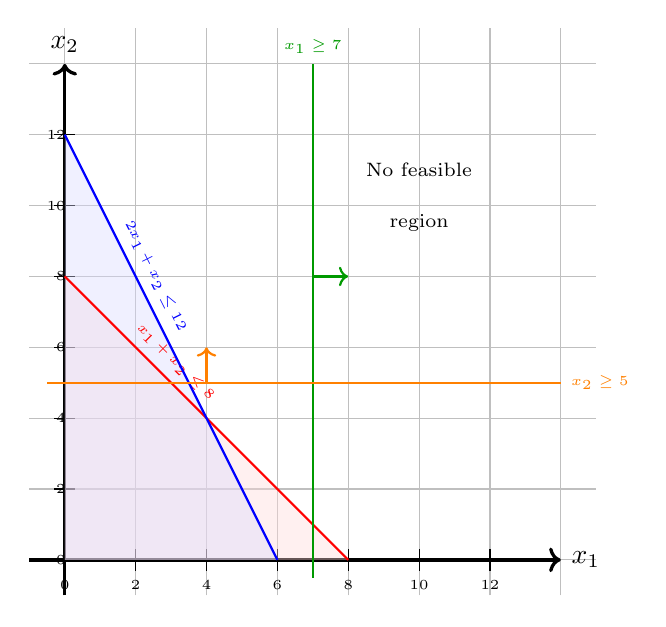
\begin{tikzpicture}[scale=0.45]
    % Grid and axes
    \draw[gray!50, thin, step=2] (-1,-1) grid (15,15);
    \draw[very thick,->] (-1,0) -- (14,0) node[right] {$x_1$};
    \draw[very thick,->] (0,-1) -- (0,14) node[above] {$x_2$};

    \foreach \x in {0,2,...,12} \draw (\x,0.3) -- (\x,-0.3) node[below] {\tiny\x};
    \foreach \y in {0,2,...,12} \draw (-0.3,\y) -- (0.3,\y) node[left] {\tiny\y};

    % Constraint regions
    \fill[red!15,opacity=0.4] (0,8) -- (8,0) -- (0,0) -- cycle;
    \fill[blue!15,opacity=0.4] (0,12) -- (6,0) -- (0,0) -- cycle;

    % Constraint lines
    \draw[red,thick] (0,8) -- node[above left, sloped] {\tiny $x_1 + x_2 \leq 8$} (8,0);
    \draw[blue,thick] (0,12) -- node[above left, sloped] {\tiny $2x_1 + x_2 \leq 12$} (6,0);
    \draw[green!60!black,thick] (7,-0.5) -- (7,14) node[above] {\tiny $x_1 \geq 7$};
    \draw[orange,thick] (-0.5,5) -- (14,5) node[right] {\tiny $x_2 \geq 5$};

    % Arrows showing required direction
    \draw[->,green!60!black,thick] (7,8) -- (8,8);
    \draw[->,orange,thick] (4,5) -- (4,6);

    % Infeasibility label
    \node[black] at (10,11) {\scriptsize No feasible};
    \node[black] at (10,9.5) {\scriptsize region};
\end{tikzpicture}
\end{document}
